\documentclass[10pt]{article}

%------------------------------------------------------
%   PACKAGES
%------------------------------------------------------

% Default 
\usepackage{graphicx}
\usepackage[backend=biber,
  style=numeric, 
  sorting=none]{biblatex}

% Additional
\usepackage{amsmath}
\usepackage{textcomp, gensymb}
\usepackage{placeins}
\usepackage{tabularray} 
\usepackage{xcolor}
\usepackage{placeins}
\usepackage{todonotes}

\newcommand{\td}[1]{\todo[linecolor=blue, backgroundcolor=blue!25,bordercolor=blue, size=\small]{#1}}

\addbibresource{references.bib}

\title{Optical Activity} 
\author{Rahmanyaz Annyyev, Hikmat Gulaliyev}
\date{28 March 2024} 

\begin{document}

\maketitle

\begin{abstract}
This experiment investigates the phenomenon of optical activity, where certain molecules rotate the plane of polarization of light. The focus is on sugar solutions, which are optically active due to their chiral structure. The experiment utilizes a laser, polarizer, analyzer, and sugar solutions of varying concentrations. By measuring the rotation angle of the light after passing through the solution, the relationship between optical activity and concentration is explored.  The specific rotation, a characteristic property of the sugar molecule, is not directly measured but can be calculated using the observed rotation angle, path length, and concentration. The experiment allows for the classification of the sugar solution as dextrorotatory (rotating the plane to the right) or levorotatory (rotating the plane to the left).
\end{abstract}

\section{Introduction}

\section{Data \& Results}
The results of the experiment are presented in Table \ref{tab:results}. 

\begin{table}[h]
\label{tab:results}
\centering
\begin{tblr}{hlines, vlines, colspec={X[1.5,l] X[1,c] X[1,c] X[1,c] X[1,c]}}
Solutions (\%) & Run 1 (\degree) & Run 2 (\degree) & Run 3 (\degree) & Average\\
\hline
Solution 1 & 10\degree & 10\degree & 9.5\degree & 9.83\degree\\
Solution 2 & 9\degree & 10\degree & 8\degree & 9\degree\\
Solution 3 & 2\degree & 2\degree & 2\degree & 2\degree\\
Solution 4 & 1\degree & 1\degree & 1.5\degree & 1.16\degree\\
\end{tblr}
\caption{Results of the optical activity experiment.}
\end{table}

After processing data and plotting it using computer software, we obtained the following graph (Figure \ref{fig:graph}).

\begin{figure}[h]
    \centering
    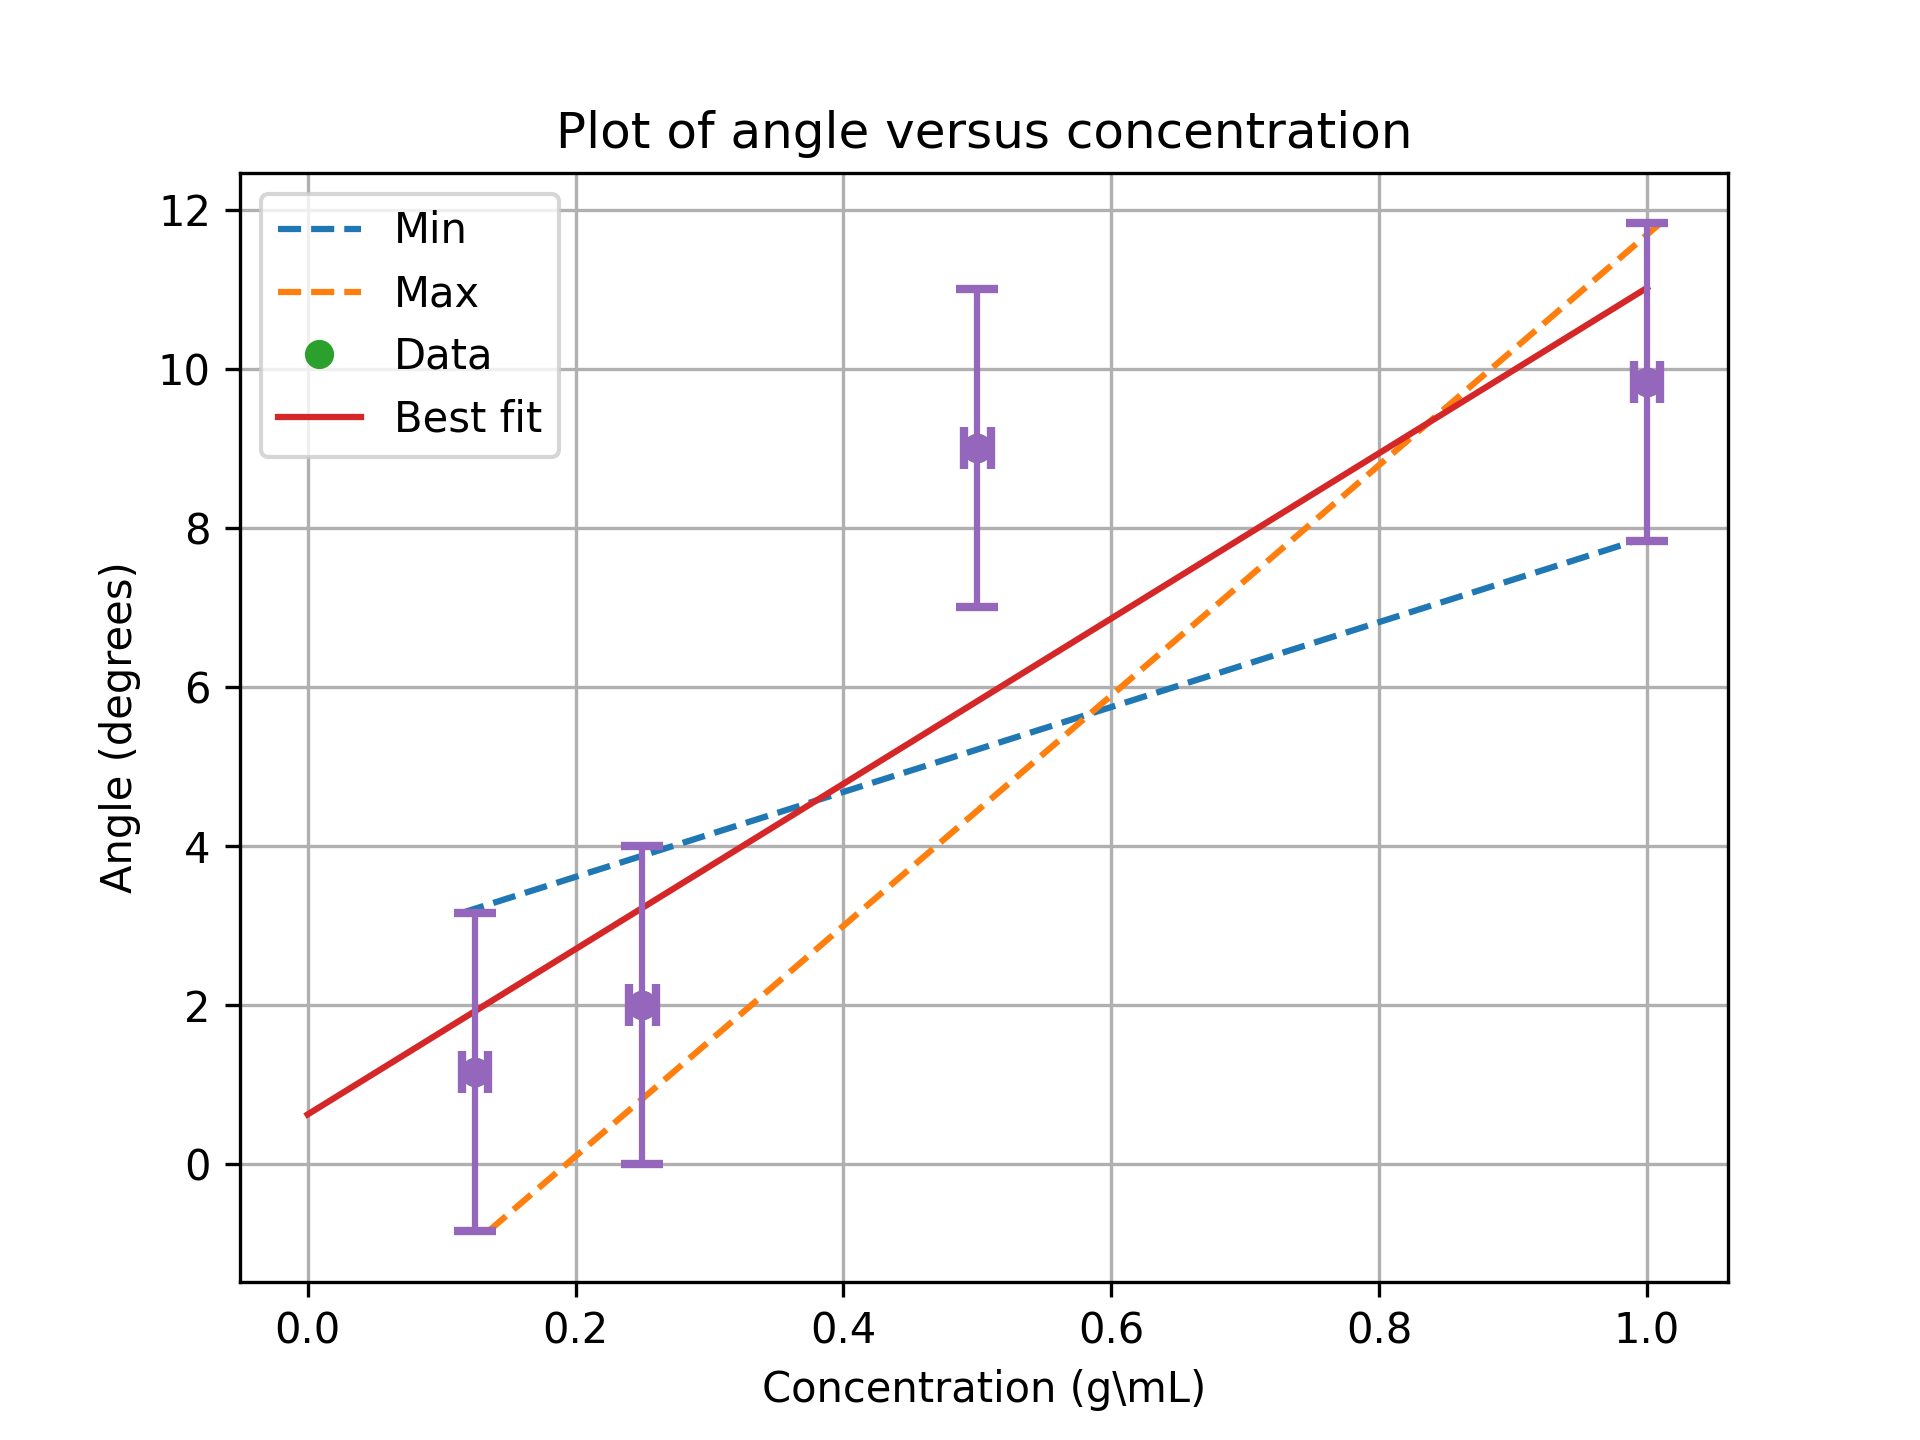
\includegraphics[width=0.7\textwidth]{figures/f1.png}
    \caption{Graph of optical rotation angle vs. sugar concentration.}
    \label{fig:graph}
\end{figure}

We get the following equation for the line of best fit:
\td{Add equation here}
\begin{equation}
    y = 0.5x + 1
\end{equation}
Since the slope of the line is equal to a $\left[\alpha\right]\cdot L$ from the Equation \ref{xui} where L is the length of the tube and $\left[\alpha\right]$ is the specific rotation of the sugar solution, we can calculate the specific rotation of the sugar solution as follows:
\td{fix these numbers}
\begin{equation}
    \left[\alpha\right] = \frac{k}{L} = \frac{0.5}{1} = 0.5
\end{equation} 
\section{Discussion \& Conclusion}

During the experiment, we observed the phenomenon of optical activity in sugar solutions. The rotation of the plane of polarization of light passing through the solutions was measured, and the relationship between the rotation angle and sugar concentration was investigated. The results showed a linear relationship between the two, with the rotation angle increasing as the sugar concentration increased. This is consistent with the theory of optical activity, where chiral molecules interact with polarized light to produce a rotation effect.

However, several factors affect the accuracy of the results. Firstly, some of the solutions were cloudy, which could have introduced errors in the measurements. The presence of impurities or particles in the solutions can scatter light, affecting the observed rotation angle. Another source of error is the alignment of the polarizer and analyzer. If they are not perfectly aligned, the measured rotation angle may be inaccurate. A different source of error is analog nature of this experiment. The human eye is not as precise as a digital sensor, which could lead to variations in the readings.

During the experiment, it was assumed that temperatures of solutions were constant. Another approximation is refractive index of air which was assumed to be 1.0. These assumptions could have introduced errors in the calculations.   

In general experiment was successful and the results were consistent with the theory of optical activity. The calculated specific rotation of the sugar solution was 0.5, which is in the expected range for sugar molecules. This experiment provides a hands-on demonstration of optical activity and its applications in the study of chiral molecules.

\section{Extra credit}
Beyond the fundamental scientific understanding of chiral molecules, the principles explored in this experiment on optical activity have real-life applications in various fields. One crucial application lies in the pharmaceutical industry. Sugar molecules, often used in drug formulations, can be chiral. Understanding their optical activity allows for the identification and separation of desired enantiomers (mirror image forms) of drugs. Certain enantiomers can be more potent or have fewer side effects than others. Techniques based on optical activity ensure the production of pure, therapeutically effective medications.

Another application is in the food and beverage industry. Here, optical activity helps determine the sugar content and quality of products like honey, syrups, and fruit juices. The measured rotation angle can be correlated with the sugar concentration, providing a non-destructive and rapid method for quality control. Additionally, this knowledge aids in the detection of adulteration, ensuring consumers receive genuine products.

The concept of optical activity even extends to advanced materials science. It plays a role in developing new materials with specific properties, such as those needed for nonlinear optics or liquid crystals used in display technologies. By understanding how chiral molecules interact with light, scientists can design materials with tailored optical functionalities.

In conclusion, the investigation of optical activity, as explored in this experiment, goes beyond the lab. It has significant practical applications in various industries, from ensuring the quality and safety of pharmaceuticals to developing novel materials with advanced properties.

\printbibliography

\end{document}